\documentclass[tikz,border=5pt]{standalone}
% Scale s = 0.017978 units/px, centred on image point (260,210), y flipped
\usetikzlibrary{calc}
\begin{document}
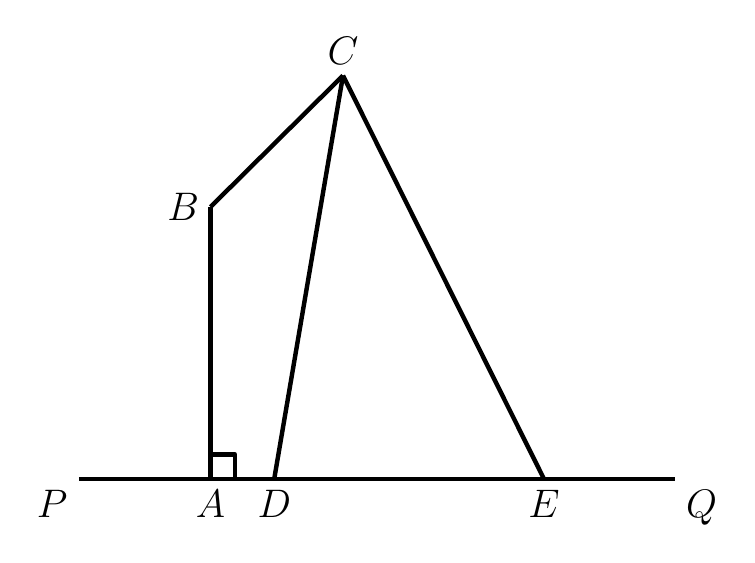
\begin{tikzpicture}[line width=1.6pt, line join=round, font=\fontsize{14}{16.8}\selectfont]

% Named points (converted from pixels; coordinates unchanged)
\coordinate (P) at (-3.793,-2.499);   % left end of baseline
\coordinate (Q) at (3.775,-2.499);    % right end of baseline
\coordinate (A) at (-2.121,-2.499);
\coordinate (B) at (-2.121,0.953);
\coordinate (C) at (-0.439,2.621);
\coordinate (D) at (-1.312,-2.499);
\coordinate (E) at (2.112,-2.499);

% Baseline PQ
\draw (P) -- (Q);

% Vertical AB
\draw (A) -- (B);

% Segment BC
\draw (B) -- (C);

% Lines from C
\draw (C) -- (D);
\draw (C) -- (E);

% Right-angle mark at A (single mark, between baseline and AB)
\draw (-2.121,-2.499) -- (-1.812,-2.499) -- (-1.812,-2.189) -- (-2.121,-2.189);

% Labels
\node[below] at (A) {$A$};
\node[below] at (D) {$D$};
\node[below] at (E) {$E$};
\node[left] at (B) {$B$};
\node[above] at (C) {$C$};
\node[below left] at (P) {$P$};
\node[below right] at (Q) {$Q$};

\end{tikzpicture}
\end{document}